\documentclass[11pt,a4paper,oneside]{report}             % Single-side
%\documentclass[11pt,a4paper,twoside,openright]{report}  % Duplex

%\PassOptionsToPackage{chapternumber=Huordinal}{magyar.ldf}
\usepackage{t1enc}
\usepackage[utf8]{inputenc}
\usepackage{amsmath}
\usepackage{amssymb}
\usepackage{enumerate}
\usepackage[thmmarks]{ntheorem}
\usepackage{graphics}
\usepackage{epsfig}
\usepackage{listings}
\usepackage{color}
\usepackage{fancyhdr}
\usepackage{lastpage}
\usepackage{anysize}
%\usepackage[magyar]{babel}
\usepackage{sectsty}
\usepackage{setspace}  % Ettol a tablazatok, abrak, labjegyzetek maradnak 1-es sorkozzel!
\usepackage[hang]{caption}
\usepackage{hyperref}

%--------------------------------------------------------------------------------------
% Main variables
%--------------------------------------------------------------------------------------
\newcommand{\vikszerzo}{Kiss Dániel Márkr}
\newcommand{\vikkonzulens}{dr.~Konzulens Elemér}
\newcommand{\vikcim}{Elektronikus terelők}
\newcommand{\viktanszek}{Méréstechnika És Információs Rendszerek Tanszék}
\newcommand{\vikdoktipus}{Önálló laboratórium 1}
\newcommand{\vikdepartmentr}{---}

%--------------------------------------------------------------------------------------
% Page layout setup
%--------------------------------------------------------------------------------------
% we need to redefine the pagestyle plain
% another possibility is to use the body of this command without \fancypagestyle
% and use \pagestyle{fancy} but in that case the special pages
% (like the ToC, the References, and the Chapter pages)remain in plane style

\pagestyle{plain}
\setlength{\parindent}{0pt} % �ttekinthet�bb, angol nyelv� dokumentumokban jellemz�
\setlength{\parskip}{8pt plus 3pt minus 3pt} % �ttekinthet�bb, angol nyelv� dokumentumokban jellemz�
%\setlength{\parindent}{12pt} % magyar nyelv� dokumentumokban jellemz�
%\setlength{\parskip}{0pt}    % magyar nyelv� dokumentumokban jellemz�

\marginsize{35mm}{25mm}{15mm}{15mm} % anysize package
\setcounter{secnumdepth}{0}
\sectionfont{\large\upshape\bfseries}
\setcounter{secnumdepth}{2}
\singlespacing
\frenchspacing

%--------------------------------------------------------------------------------------
%	Setup hyperref package
%--------------------------------------------------------------------------------------
\hypersetup{
    bookmarks=true,            % show bookmarks bar?
    unicode=false,             % non-Latin characters in Acrobat�s bookmarks
    pdftitle={\vikcim},        % title
    pdfauthor={\vikszerzo},    % author
    pdfsubject={\vikdoktipus}, % subject of the document
    pdfcreator={\vikszerzo},   % creator of the document
    pdfproducer={Producer},    % producer of the document
    pdfkeywords={keywords},    % list of keywords
    pdfnewwindow=true,         % links in new window
    colorlinks=true,           % false: boxed links; true: colored links
    linkcolor=black,           % color of internal links
    citecolor=black,           % color of links to bibliography
    filecolor=black,           % color of file links
    urlcolor=black             % color of external links
}

%--------------------------------------------------------------------------------------
% Set up listings
%--------------------------------------------------------------------------------------
\lstset{
	basicstyle=\scriptsize\ttfamily, % print whole listing small
	keywordstyle=\color{black}\bfseries\underbar, % underlined bold black keywords
	identifierstyle=, 					% nothing happens
	commentstyle=\color{white}, % white comments
	stringstyle=\scriptsize\sffamily, 			% typewriter type for strings
	showstringspaces=false,     % no special string spaces
	aboveskip=3pt,
	belowskip=3pt,
	columns=fixed,
	backgroundcolor=\color{lightgray},
} 		
\def\lstlistingname{lista}	

%--------------------------------------------------------------------------------------
%	Some new commands and declarations
%--------------------------------------------------------------------------------------
\newcommand{\code}[1]{{\upshape\ttfamily\scriptsize\indent #1}}

% define references
\newcommand{\figref}[1]{\ref{fig:#1}.}
\renewcommand{\eqref}[1]{(\ref{eq:#1})}
\newcommand{\listref}[1]{\ref{listing:#1}.}
\newcommand{\sectref}[1]{\ref{sect:#1}}
\newcommand{\tabref}[1]{\ref{tab:#1}.}

\DeclareMathOperator*{\argmax}{arg\,max}
%\DeclareMathOperator*[1]{\floor}{arg\,max}
\DeclareMathOperator{\sign}{sgn}
\DeclareMathOperator{\rot}{rot}
\definecolor{lightgray}{rgb}{0.95,0.95,0.95}

\author{\vikszerzo}
\title{\viktitle}
\includeonly{
	titlepage,%
	introduction,%
	chapter1,%
	chapter2,%
	chapter3,%
	chapter4,%
}
%--------------------------------------------------------------------------------------
%	Setup captions
%--------------------------------------------------------------------------------------
\captionsetup[figure]{
%labelsep=none,
%font={footnotesize,it},
%justification=justified,
width=.75\textwidth,
aboveskip=10pt}

\renewcommand{\captionlabelfont}{\small\bf}
\renewcommand{\captionfont}{\footnotesize\it}

%--------------------------------------------------------------------------------------
% Table of contents and the main text
%--------------------------------------------------------------------------------------
\begin{document}
\singlespacing
\pagenumbering{arabic}
\onehalfspacing
\begin{titlepage}
    \begin{center}
        
\includegraphics[width=60mm,keepaspectratio]{../images/BMElogo.png}\\
        \vspace{0.3cm}
        \textbf{Budapest University of Technology and Economics}\\
        \textmd{Faculty of Electrical Engineering and Informatics}\\
        \textmd{\viktanszek}\\[5cm]

        \vspace{0.4cm}
        {\huge \bfseries \vikcim}\\[0.8cm]
        \vspace{0.5cm}
        \textsc{\Large \vikdoktipus}\\[4cm]

        \begin{tabular}{cc}
            \makebox[7cm]{\emph{Author}} & \makebox[7cm]{\emph{Supervisor}} \\
            \makebox[7cm]{\vikszerzo}    & \makebox[7cm]{\vikkonzulens}
        \end{tabular}

        \vfill
        {\large \today}
    \end{center}
\end{titlepage}



\tableofcontents\vfill
\chapter{Introduction}

Smartphones have become a defining part of our days. By now we can't even imagine our everyday life without them. We read e-mails, browse the Internet or monitor daily exchange rates. Now we can do all important things with our phones. Listening to music and watching series, but in terms of photography and video capabilities, they are not far behind cameras designed for professional purposes. Their computing capacity has grown exponentially over the years. The quality of camera systems is also undergoing significant progress every year.Perhaps this is why many people say that the development of telephones is starting to slow down. This industry has reached its peak.

At the time, in 2007, the iPhone was considered a huge world sensation and now we know it was a world-changing announcement. At the time of writing this report, there are several reports that Apple is working on the introduction of a similarly large and decisive new product line. The so-called Apple AR/VR glasses. Only time will tell if this really happened until then I thought that it would be a great advance if I started familiarising with this technology. If this will be the next "touchscreen phone era", I thought it would be worthwhile to start dealing with it in time. Regardless, I have long been interested in the technology's operating principle and scope of use. From the consumer side, what kind of application possibilities does augmented reality technology have? At that time, I wanted to implement a similar augmented reality-like navigation system in my own high school navigation application. Unfortunately, I did not know about the existence of these technologies at the time.

As I mentioned in the first paragraph, today's phones have a huge computing capacity. This is also why it is possible for such augmented reality applications to run on our phones. Based on the 1 or better case 2 or 3 lenses placed in the phone, it can measure the 3D depth of each scenario. There are phones, such as the iPhone 13 Pro, which have a laser LiDAR sensor placed specifically for this purpose. In the 2010s, many devices with similar technology came out, such as Microsoft's Kinect developed for the X-Box 360 console. It is also worth mentioning Google Glass developed by Google or HoloLens and HoloLens 2 marketed by Microsoft. Unfortunately, the former mentioned Google Glass was not an undivided success and in 2023 the sale of the glasses was discontinued.

Last but not least, it is important to mention the Oculus Quest 2 VR headset introduced by Meta and the computer use and games based on it. In addition, the Metaverse, announced by Meta 2 years ago, is also an important milestone in the life of virtual reality and therefore also in the life of augmented reality.

As the examples above clearly reflect, it will be an important and presumably defining technology in the future. In light of this, during my self-lab, I got to know the ARKit and RealityKit developed and used by Apple. And with the help of the frameworks, I developed an augmented reality application displaying economic metrics. And during the report I used LaTex, because I felt it was time to familiarize myself with this kind of documentation language.

\chapter{Introduction}

Smartphones have become a defining part of our days. By now we can't even imagine our everyday life without them. We read e-mails, browse the Internet or monitor daily exchange rates. Now we can do all important things with our phones. Listening to music and watching series, but in terms of photography and video capabilities, they are not far behind cameras designed for professional purposes. Their computing capacity has grown exponentially over the years. The quality of camera systems is also undergoing significant progress every year.Perhaps this is why many people say that the development of telephones is starting to slow down. This industry has reached its peak.

At the time, in 2007, the iPhone was considered a huge world sensation and now we know it was a world-changing announcement. At the time of writing this report, there are several reports that Apple is working on the introduction of a similarly large and decisive new product line. The so-called Apple AR/VR glasses. Only time will tell if this really happened until then I thought that it would be a great advance if I started familiarising with this technology. If this will be the next "touchscreen phone era", I thought it would be worthwhile to start dealing with it in time. Regardless, I have long been interested in the technology's operating principle and scope of use. From the consumer side, what kind of application possibilities does augmented reality technology have? At that time, I wanted to implement a similar augmented reality-like navigation system in my own high school navigation application. Unfortunately, I did not know about the existence of these technologies at the time.

As I mentioned in the first paragraph, today's phones have a huge computing capacity. This is also why it is possible for such augmented reality applications to run on our phones. Based on the 1 or better case 2 or 3 lenses placed in the phone, it can measure the 3D depth of each scenario. There are phones, such as the iPhone 13 Pro, which have a laser LiDAR sensor placed specifically for this purpose. In the 2010s, many devices with similar technology came out, such as Microsoft's Kinect developed for the X-Box 360 console. It is also worth mentioning Google Glass developed by Google or HoloLens and HoloLens 2 marketed by Microsoft. Unfortunately, the former mentioned Google Glass was not an undivided success and in 2023 the sale of the glasses was discontinued.

Last but not least, it is important to mention the Oculus Quest 2 VR headset introduced by Meta and the computer use and games based on it. In addition, the Metaverse, announced by Meta 2 years ago, is also an important milestone in the life of virtual reality and therefore also in the life of augmented reality.

As the examples above clearly reflect, it will be an important and presumably defining technology in the future. In light of this, during my self-lab, I got to know the ARKit and RealityKit developed and used by Apple. And with the help of the frameworks, I developed an augmented reality application displaying economic metrics. And during the report I used LaTex, because I felt it was time to familiarize myself with this kind of documentation language.

\chapter{Current techologies}

Before I started the development of the application I have done a research period to have a better overview of the current market. There are several frameworks to choose from to start developing augmented reality applications. The most used AR frameworks are Google ARCore, Apple ARKit and RealityKit, Simple CV and Unity AR Foundation.
I ended up using Apple ARKit to build my app. I've been working with iOS development for several years and I'm sure with the Swift language as well.

\include{chapter2}
\chapter{Development}

\section{Overview}
For the development phase of the project I used Apple's XCode integrated developer environment(IDE) as the main developer platform for iOS and ARKit development. For testing I used an iPhone 11 with dual camera system.
I have also version controled the whole development process using git and publishing it on GitHub. Not only the source code can be found there but also the documentation of this project as I have writen it using \LaTeX{}.

\section{APILayer Rest API}

The fundamental part of the application is the data it displays. For retriving the displayed informations I used APILayer's Exchange Rates Data API an open and available for free financial API.  The only problem is that you can only do 250 queries per month in the free version. I used 2 endpoints. The first is '/convert'. With this endpoint, we have any amount conversion from one currency to another. The output of this enpoint is the following JSON.

\begin{lstlisting}[frame=single,float=!ht,caption=JSON from /convert endpoint, label=listing:Bibtex]
  {
    "success": true,
    "query": {
        "from": "EUR",
        "to": "HUF",
        "amount": 1
    },
    "info": {
        "timestamp": 1682930463,
        "rate": 373.180303
    },
    "date": "2023-05-01",
    "result": 373.180303
  }
\end{lstlisting}

The other endpoint used is '/fluctuation'. This endpoint returns the fluctuation data between specified dates. The data can be for all available currencies or for a specific set.
\begin{lstlisting}[frame=single,float=!ht,caption=JSON from /fluctuation endpoint, label=listing:Bibtex]
{
  "base": "EUR",
  "end_date": "2018-02-26",
  "fluctuation": true,
  "rates": {
    "JPY": {
      "change": 0.0635,
      "change_pct": 0.0483,
      "end_rate": 131.651142,
      "start_rate": 131.587611
    },
    "USD": {
      "change": 0.0038,
      "change_pct": 0.3078,
      "end_rate": 1.232735,
      "start_rate": 1.228952
    }
  },
  "start_date": "2018-02-25",
  "success": true
}
\end{lstlisting}

\section{SwiftUI}

SwiftUI is Apple's brand new framework for building user interfaces for iOS, tvOS, macOS, and watchOS. Apple introduced SwiftUI in 2019 and the framework has been evolving ever since. Unlike UIKit, SwiftUI is a cross-platform framework. The key difference with UIKit and AppKit is that SwiftUI defines the user interface declaratively, not imperatively. What does that mean?

Using UIKit you create views to build the view hierarchy of your application's user interface. That is not how SwiftUI works. SwiftUI provides developers with an API to declare or describe what the user interface should look like. SwiftUI inspects the declaration or description of the user interface and converts it to your application's user interface. SwiftUI does the heavy lifting for you.

One of the most challenging aspects of user interface development is synchronizing the application's state and its user interface. Every time the application's state changes, the user interface needs to update to reflect the change. During the development phase, this was a challenge that had to be overcome. Despite the fact that I have already used and developed an iOS application with SwiftUI, it was excellent practice to deepen my knowledge of user state management. I used ObservableObjects to solve this problem.

I used a common state management technique, the MVC pattern, to control the data and model. MVC (Model-View-Controller) is a pattern in software design commonly used to implement user interfaces, data, and controlling logic. It emphasizes a separation between the software's business logic and display. This "separation of concerns" provides for a better division of labor and improved maintenance. Sticking to convention, I created a CurrencyController, CurrencyView and a CurrencyModell class. The CurrencyModel class contains the generated 3D models and their associated values. The task of the CurrencyController class is to query the data and update the information displayed on the View. In the CurrencyView class, it deals with the code defining the appearance of the application and the display of the given dataset.


\section{ARKit and RealityKit}

To operate augmented reality and display the 3D generated graph, I used the ARKit and RealityKit frameworks provided by Apple.

The CurrencyARViewContainer is responsible for displaying the AR view.

\begin{lstlisting}
struct CurrencyARViewContainer: UIViewRepresentable {
    
    @StateObject var controler:CurrencyController
    
    func makeUIView(context: Context) -> ARView{
        AR.view = ARView(frame: .zero)
        return AR.view
    }
    
    func updateUIView(_ uiView: ARView, context: Context) {
        print("updating view - (controler.timerHappened)")
        uiView.scene.anchors.removeAll()
        ...
    }
}
\end{lstlisting}

To generate the texts and columns, I used the .generateBox() and .generateText() functions of the built-in MeshResource class.
The MeshResource class stores the points defining the shapes. In order for this to become a 3D model, a texture must also be specified. I used the SimpleMaterial() function for this.
We also need an AnchorEntity, which defines the center of our model in the 3D world.
After defining these variables, we can create the ModelEntity and place it in the AR world using the AnchorEntity.

\begin{lstlisting}
    func updateUIView(_ uiView: ARView, context: Context) {
        uiView.scene.anchors.removeAll()
        
        let cylinderMeshResource = MeshResource.generateBox(...)
        
        let myMaterial = SimpleMaterial(...)
        let radians = 90.0 * Float.pi / 180.0
            
        let kozeppont = AnchorEntity(world: SIMD3(x: 0.0, y: 0.0, z: 0.0))
        let axisXEntity = ModelEntity(mesh: cylinderMeshResource, materials: ...)
        
        let coneXEntity = ModelEntity(mesh: coneMeshResource, materials: ...)
        coneXEntity.orientation = simd_quatf(...)
        
        axisXEntity.addChild(coneXEntity)
        coneXEntity.setPosition(...)
        
        kozeppont.addChild(axisXEntity)
        uiView.scene.addAnchor(kozeppont)
        ...
    }
\end{lstlisting}

To be able to move the different elements together, all 3D models are children of the axes. Thus, if the axis moves, the connected elements will also move due to the parent-child relationship. In its current version, MeshResource does not support the generation of cones by default, so I was able to achieve this by using an external library package. After importing the RealityGeometries library, I was able to easily generate cones, which I eventually used to draw axes.

\chapter{Presentation of finished work}

In this section I will present and showcase my finished appliction. I will include screenshots to have a better representation and understanding for the reader.
The camera function in the application allows you to capture the current state of the graphs, which in this case came in handy for documentation.

\begin{figure}[!ht]
    \centering
    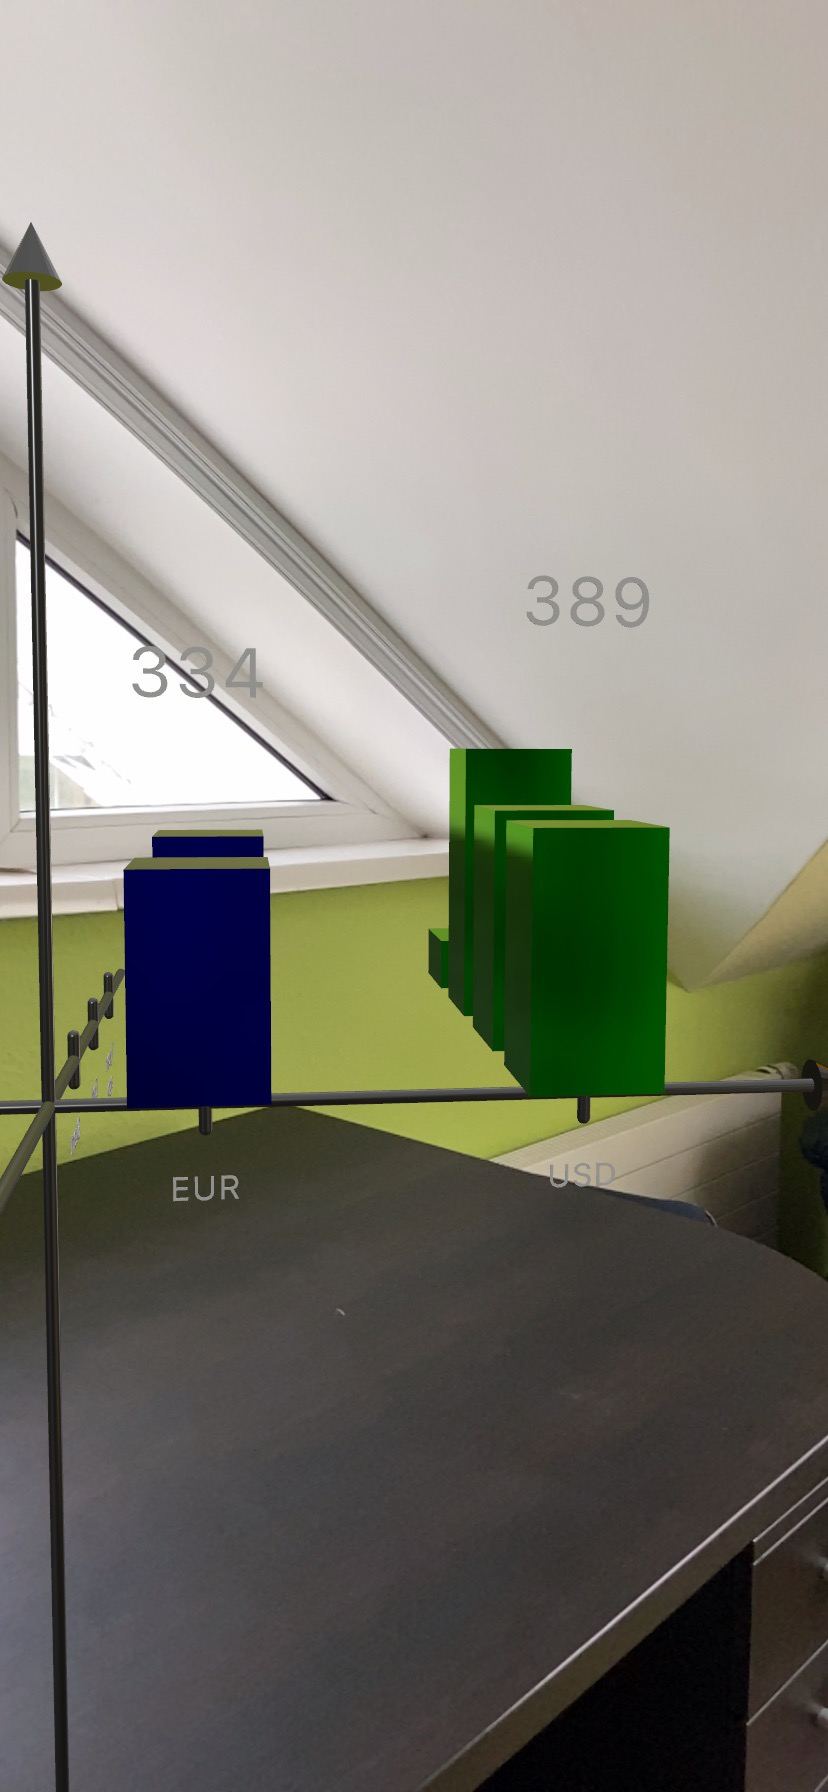
\includegraphics[height=67mm, keepaspectratio]{../images/front.jpeg}\hspace{1cm}
    %\caption{The main screen of the application.}
    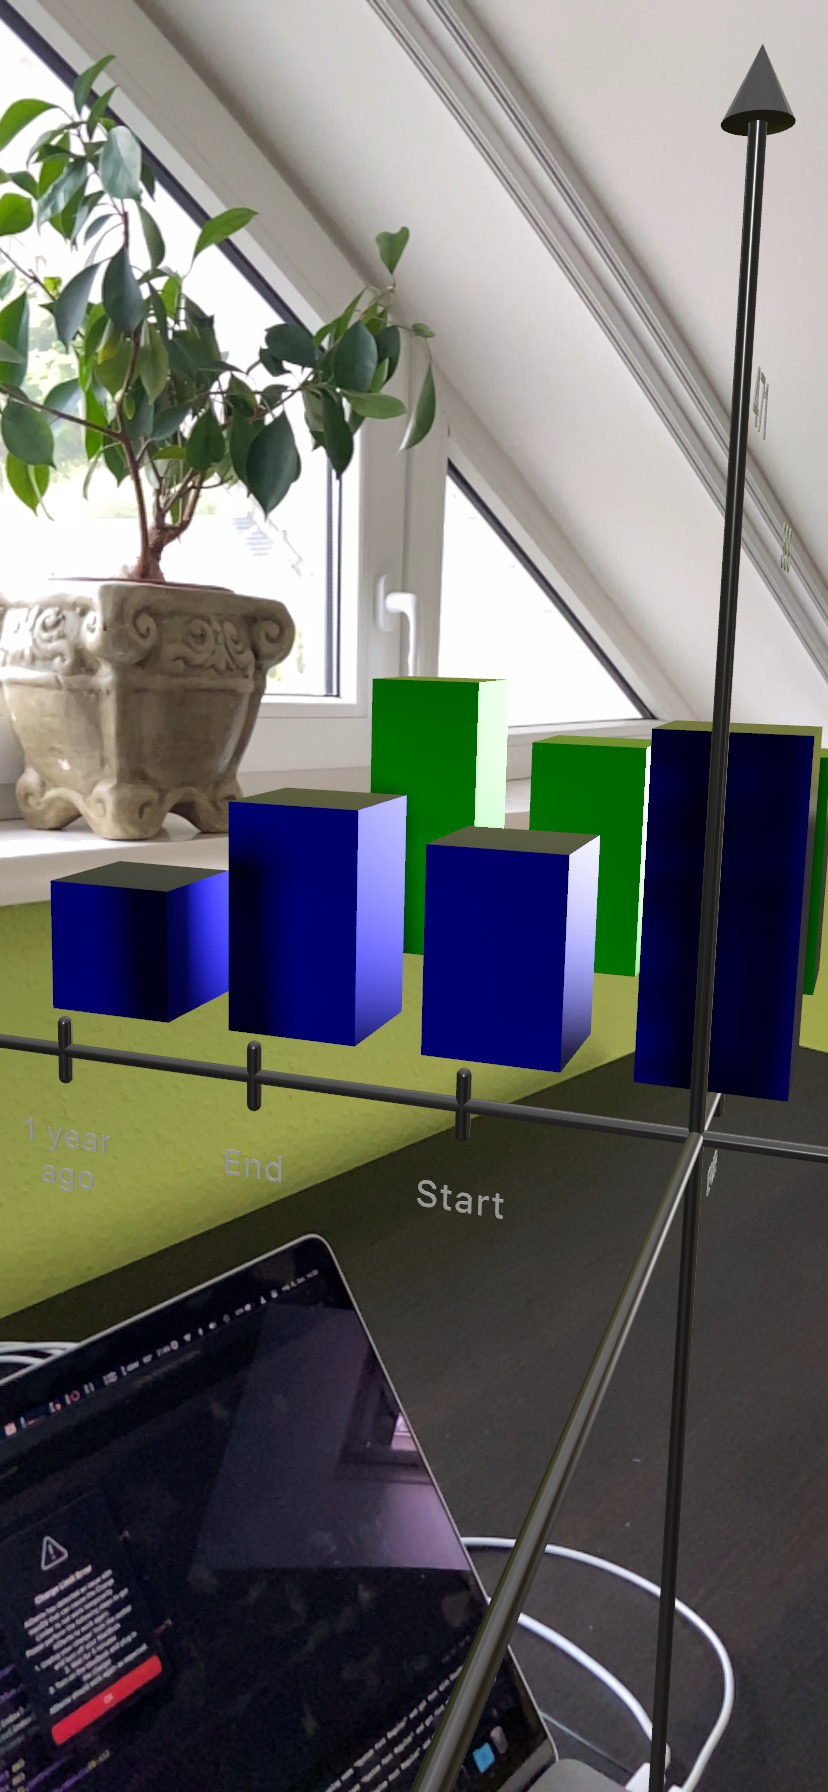
\includegraphics[height=67mm, keepaspectratio]{../images/side.jpeg}\\\vspace{5mm}
    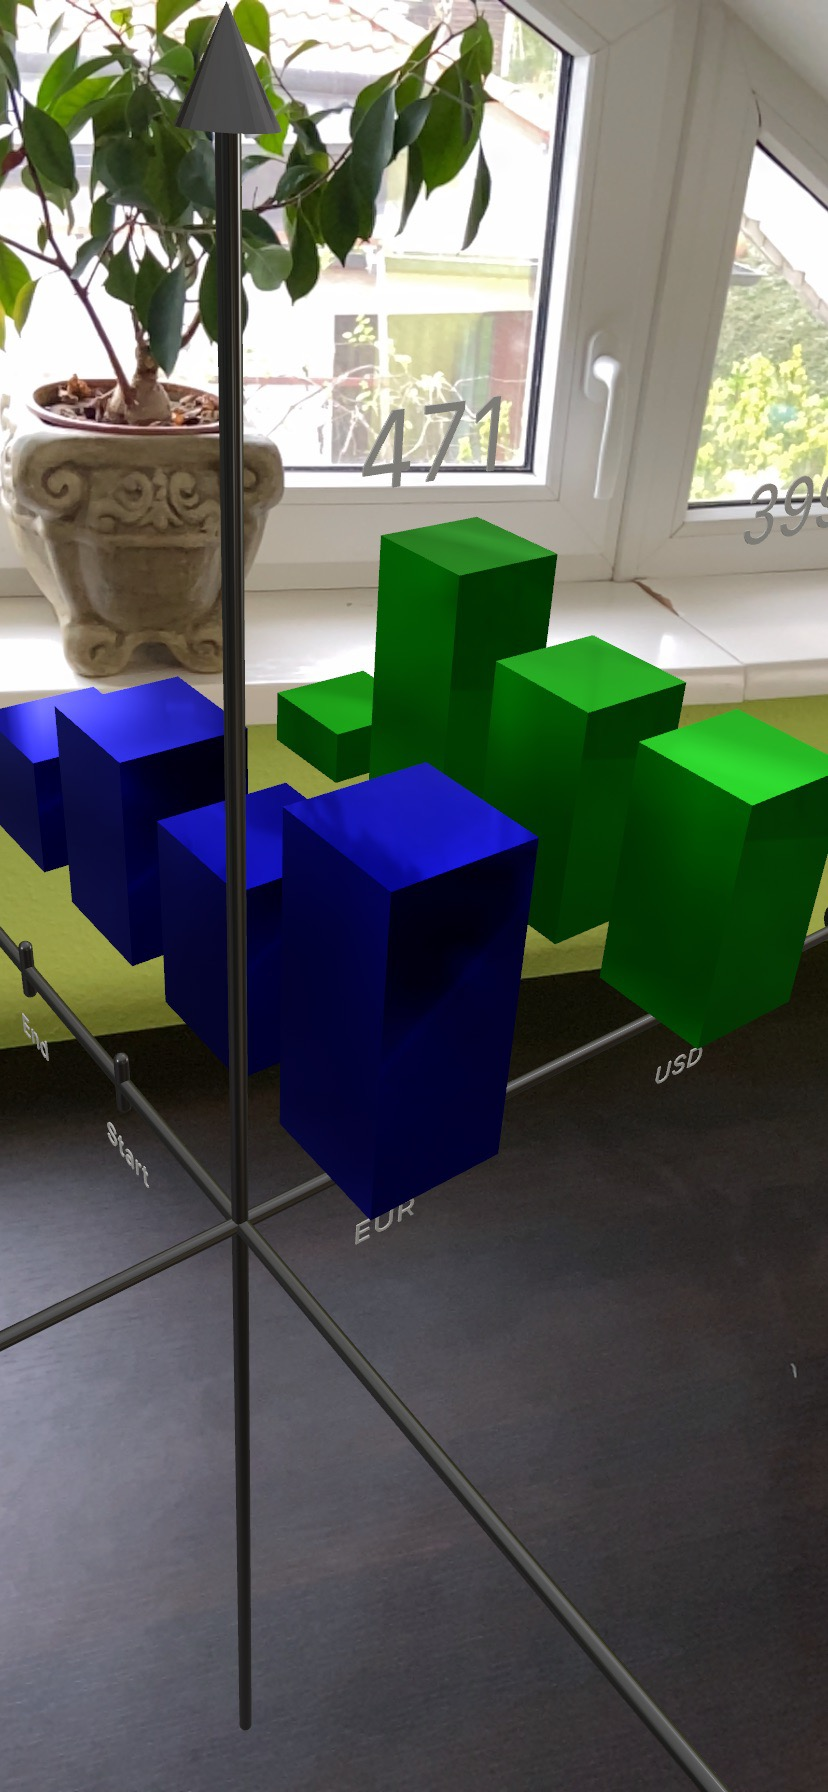
\includegraphics[height=67mm, keepaspectratio]{../images/top.jpeg}\hspace{1cm}
    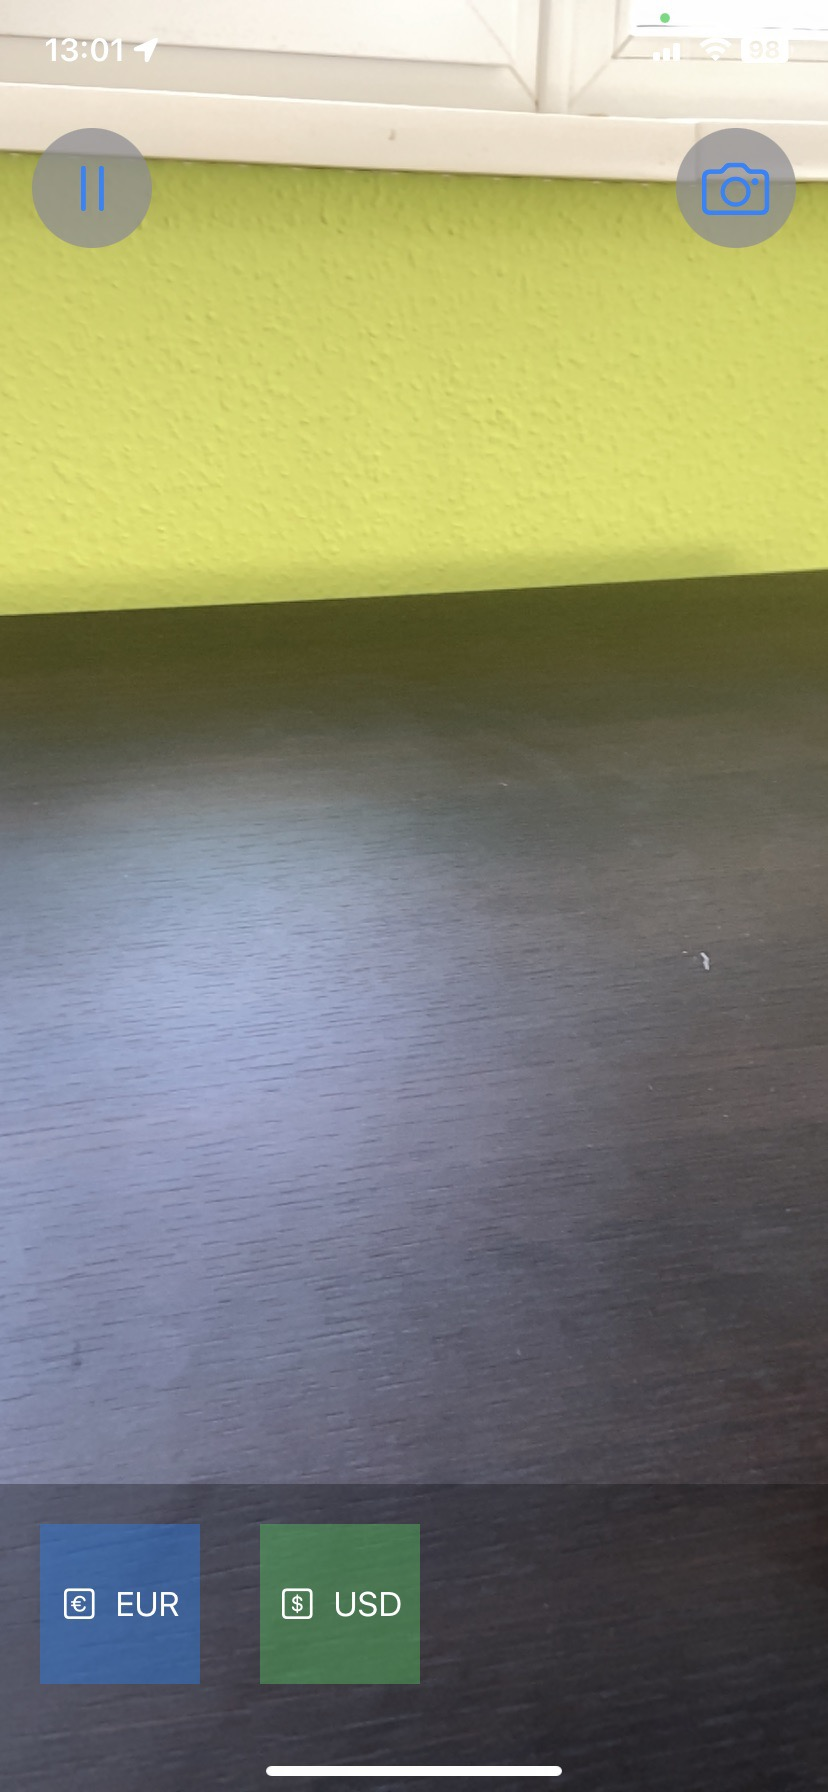
\includegraphics[height=67mm, keepaspectratio]{../images/selector.jpeg}
    \caption{Scenarios of the application}
    \label{fig:HVSpaces}
\end{figure}


As the attached images clearly show, the virtual 3D graph can be easily walked around and viewed from different angles, thereby giving users a new comparative perspective. It is possible to move and rotate the entire graph, as well as move the current exchange rate columns to make it easier to compare with other metrics. The move and rotate functions are only available in Spectate mode, for this you have to stop Live mode (or otherwise start Live mode) by pressing the button located in the upper left corner.

Currently, 2 currencies are available in the application, but of course this can be easily expanded at any time in the future. These two are EUR to HUF and USD to HUF. These can be displayed after selection and confirmation from the bottom bar. If the given exchange rate is already placed, it can no longer be added to the graph twice.



\begin{figure}[!ht]
    \centering
    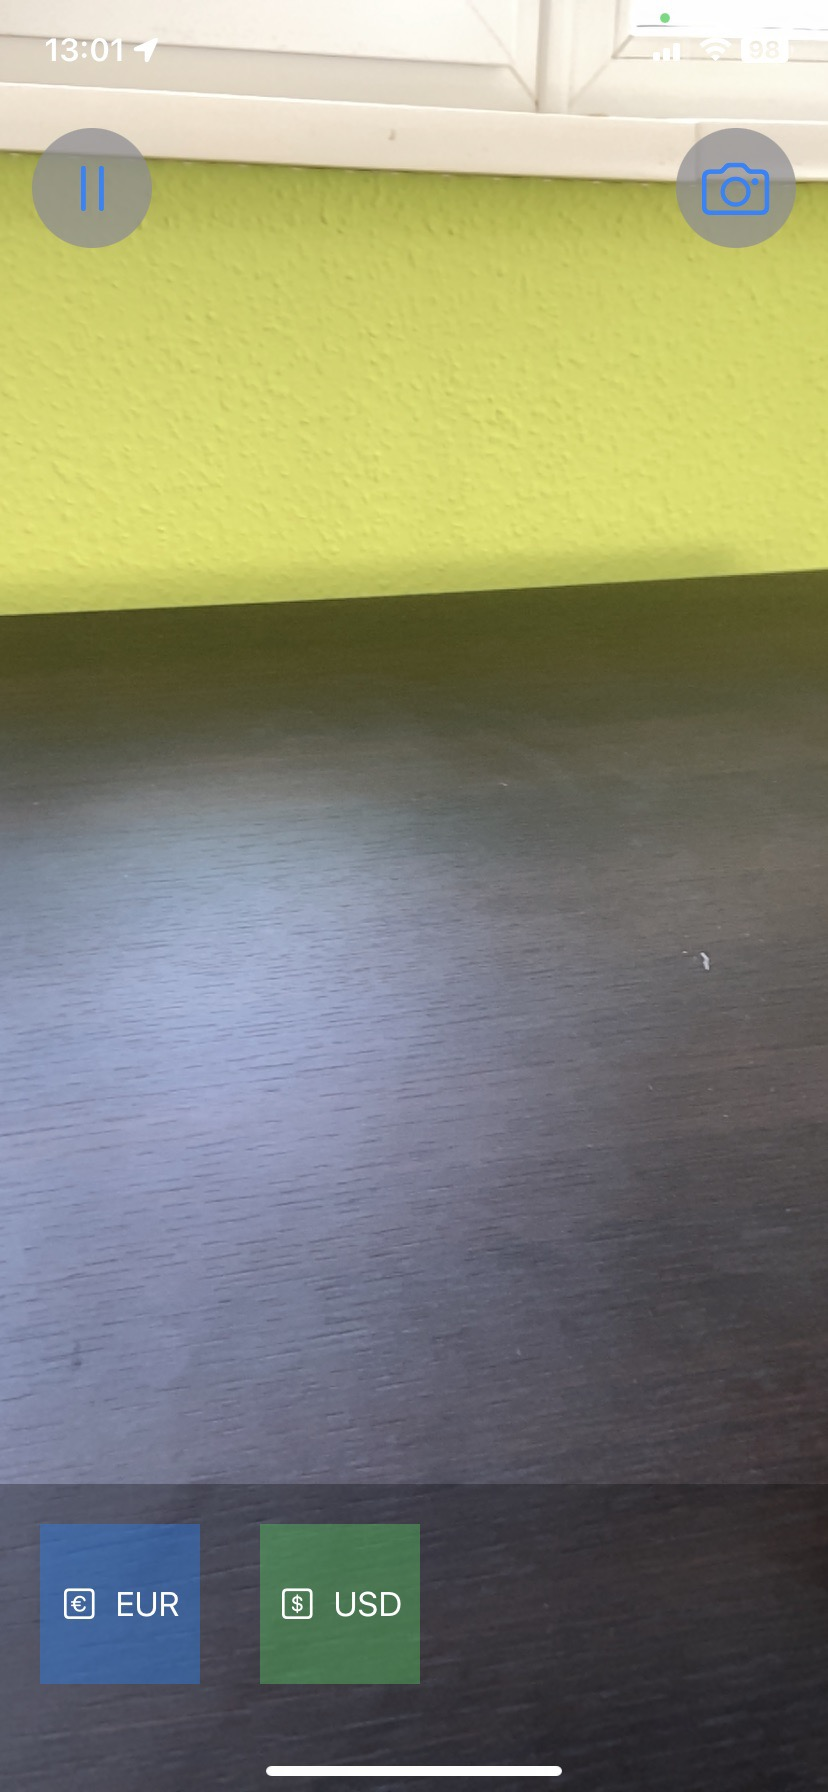
\includegraphics[height=67mm, keepaspectratio]{../images/selector.jpeg}\hspace{1cm}
    %\caption{The main screen of the application.}
    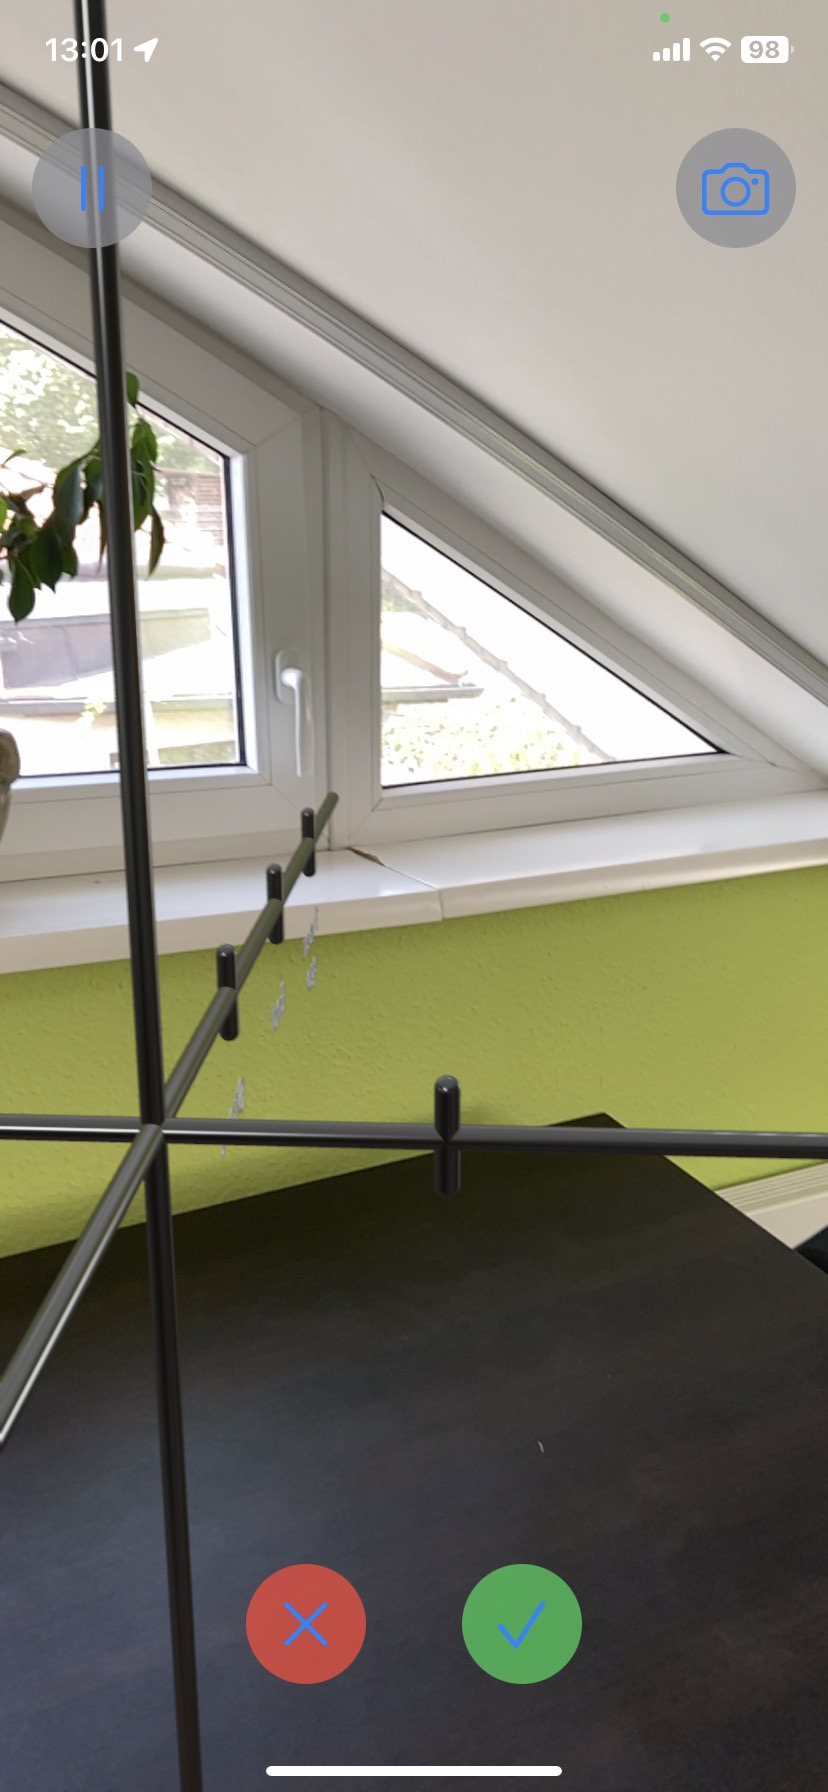
\includegraphics[height=67mm, keepaspectratio]{../images/megerosites.jpeg}\\\vspace{5mm}
    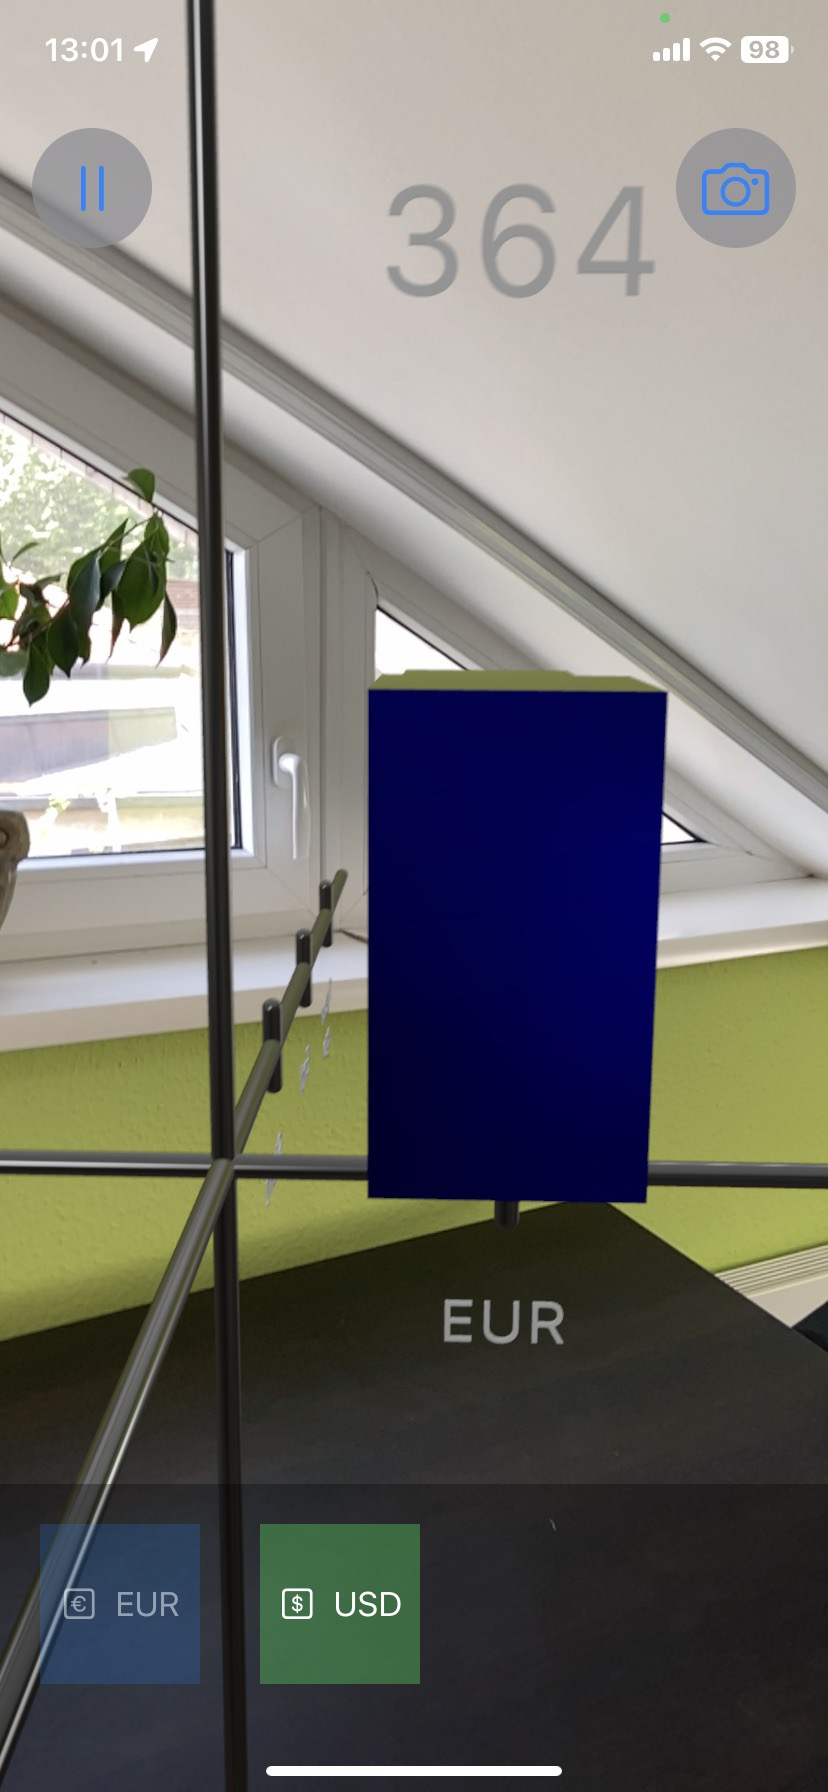
\includegraphics[height=67mm, keepaspectratio]{../images/not_available.jpeg}%\hspace{1cm}
    \caption{User interface}
    \label{fig:HVSpaces}
\end{figure}


%\listoffigures\addcontentsline{toc}{chapter}{�br�k jegyz�ke}
%\listoftables\addcontentsline{toc}{chapter}{T�bl�zatok jegyz�ke}

\bibliography{mybib}
\addcontentsline{toc}{chapter}{Irodalomjegyzék}
\bibliographystyle{plain}

\include{appendices}

\label{page:last}
\end{document}
